\documentclass[onecolumn, draftclsnofoot,10pt, compsoc]{IEEEtran}
\usepackage{graphicx}
\usepackage{url}
\usepackage{setspace}
\usepackage{caption}

\usepackage{geometry}
\geometry{textheight=9.5in, textwidth=7in}


% 1. Fill in these details
\def \CapstoneTeamName{		    Nitro Chatbot}
\def \CapstoneTeamNumber{		63}
\def \GroupMemberOne{			Jack Barnes}
\def \GroupMemberTwo{			Sarun Pitaksuteephong}
\def \GroupMemberThree{			Cheng Xie}
\def \CapstoneProjectName{		ChatBot for Load Balancer Infrastructure}
\def \CapstoneSponsorCompany{	OSU Information Services}
\def \CapstoneSponsorPerson{	Stacy Brock}

% 2. Uncomment the appropriate line below so that the document type works
\def \DocType{	%Problem Statement
				%Requirements Document
				%Technology Review
				%Design Document
				Progress Report
				}

\newcommand{\NameSigPair}[1]{\par
\makebox[2.75in][r]{#1} \hfil 	\makebox[3.25in]{\makebox[2.25in]{\hrulefill} \hfill		\makebox[.75in]{\hrulefill}}
\par\vspace{-12pt} \textit{\tiny\noindent
\makebox[2.75in]{} \hfil		\makebox[3.25in]{\makebox[2.25in][r]{Signature} \hfill	\makebox[.75in][r]{Date}}}}
% 3. If the document is not to be signed, uncomment the RENEWcommand below
\renewcommand{\NameSigPair}[1]{#1}

%%%%%%%%%%%%%%%%%%%%%%%%%%%%%%%%%%%%%%%
\begin{document}
\begin{titlepage}
    \pagenumbering{gobble}
    \begin{singlespace}
    	% 4. If you have a logo, use this includegraphics command to put it on the coversheet.
    	%\includegraphics[height=4cm]{logo-small-notext.png}
        \hfill 
        \par\vspace{.2in}
        \centering
        \scshape{
            \huge CS Capstone \DocType \par
            {\large\today}\par
            \vspace{.5in}
            \textbf{\Huge\CapstoneProjectName}\par
            \vfill
            %\includegraphics[height=8cm]{logo-small-notext.png}
            \vfill
            {\large Prepared for}\par
            \Huge \CapstoneSponsorCompany\par
            \vspace{5pt}
            {\Large\NameSigPair{\CapstoneSponsorPerson}\par}
            {\large Prepared by }\par
            Group\CapstoneTeamNumber\par
            % 5. comment out the line below this one if you do not wish to name your team
            \CapstoneTeamName\par 
            \vspace{5pt}
            {\Large
                \NameSigPair{\GroupMemberOne}\par
                \NameSigPair{\GroupMemberTwo}\par
                \NameSigPair{\GroupMemberThree}\par
            }
            \vspace{20pt}
        }
        \begin{abstract}
        % 6. Fill in your abstract
        The purpose of Nitro Chatbot is to provide a quick and highly accessible interface for users to access the status and modify configurations for their load balanced resources. Nitro Chatbot aims to provide a simple and quick interface for users to access NetScaler configurations by operating as a Chatbot within Microsoft Teams. The team completed all the nessicary documentation for Fall Term and has client approval to move forward with the project.
        \end{abstract}     
    \end{singlespace}
\end{titlepage}
\newpage
\pagenumbering{arabic}
%\tableofcontents
% 7. uncomment this (if applicable). Consider adding a page break.
%\listoffigures
%\listoftables
\clearpage
\textbf{Change History}\par

\begin{tabular}{ p{1in} p{1in} p{4in} }
 \textbf{Revision} & \textbf{Date} & \textbf{Changes} \\
 \hline
 1.0 & 12/6/2019 
 & - \\
 \hline
\end{tabular}

\clearpage

% 8. now you write!
\section{Project Information}
\subsection{Purpose}
%briefly recap the project purposes
The purpose of Nitro Chatbot is to provide a quick and highly accessible interface for users to access the status and modify configurations for their load balanced resources. 

Oregon State University uses Citrix NetScaler hardware to load balancing as a service to various departments.
Load balancing allows incoming network requests to be spread among a pool of redundant servers, increasing responsiveness and availability.

Common tasks for users with load balanced resources include querying the status of servers, enabling or disabling the servers, and updating offloaded certificates.
The current method for performing these tasks is cumbersome and inefficient.
By providing an accessible interface, users will be able to more easily perform these common tasks.
\subsection{Goals}
%briefly recap the project goals
Nitro Chatbot aims to provide a simple and quick interface for users to access NetScaler configurations by operating as a Chatbot within Microsoft Teams.
Microsoft Teams is a chat application designed for an enterprise environment and is current in use by Oregon Sate University.

To provide this solution, 2 component softwares will be developed.
The first software, known as the Chatbot, will be deployed to AWS (Amazon Web Services).
It will accept direct messages from users within Teams.
The user will need to authenticate through OSU's federated login system (using the SAML2 protocol).
Messages will be parsed as commands and forwarded to the second component software, the Relay.

The Relay, existing within the university's firewall, will translate the response into a NITRO API query (the NetScaler's REST API).
The response will then be translated back and transmitted to the ChatBot, which will display the response to the user within 60 seconds of the original request.

Nitro Chatbot will be essentially always available, continuously running in the cloud, awaiting messages from users.
It will operate in a non-blocking fashion, always accepting messages from users, and replying to the user when it receives a response from the Relay.

The Chatbot and the Relay will be written with Node.js. The Chatbot will use Botkit Framework for chatbot functionality and to assist with the integration with Microsoft Teams.

Development of Nitro Chatbot will utilize a Continuous Integration / Continuous Deployment (CI/CD) pipeline.
Jasmine unit tests will be written during development, and a Jenkins instance will be used to automatically run the tests.

A system of deployment will also be created to deploy the Chatbot into AWS with Cloud Development Kit (CDK) and Cloudformation.
CloudWatch will be used to remotely log user interactions in a persistent manner. By using CloudWatch, an inbuilt administrative interface can be used to audit logs.

\section{Project State}
\subsection{Progress}
%describe where you are currently on the project,
We have completed our initial documentation (Problem Statement, Requirements Document, and Design Document) and each document has had at least one revision.
After our last meeting, we have our client's approval to begin implementation.

Over the winter break, one team member will be working on prototyping some aspects of the program.
Through prototyping, the team hopes to gain more understanding about which authentication flow will work best to provide security and usability.

\subsection{Problems}
%describe any problems that have impeded your progress, with any solutions you have
The major problem that we've had with designing our implementation of Nitro Chatbot is with user authentication.
Originally, the requirements called for leveraging the known user identity from within Microsoft Teams.
As Microsoft Teams is an authenticated environment, we can be assured the identity of the user.
However the NetScaler needs it's own authentication for users to be able to access it.
To allow users to access configurations without re-authenticating, sensitive credentials would need to be stored.
This creates an issue with security, which is of primary concern due to the sensitive nature of the load balancer.

Instead, the team decided it would be appropriate to ask users to authenticate once and to store the authentication token for a reasonable time (likely 30 minutes).
Users needing to complete a series of tasks would need to authenticate only once at the very start.
The team and client found this to be a reasonable compromise.

The second issue the team encountered was with access to a NetScaler to be able to test API calls against.
Having access to a way to test these API calls it critical to understanding which authentication flows will be able to be implemented in Nitro ChatBot.
Having researched the NITRO API documentation, the team is fairly confident that the proposed design will be able to work.
However, doubt still exists as the team hasn't be able to perform concrete tests translating a SAML2 authentication flow through an intermediary.
Access to a NetScaler would also allow the team to test configurations and other API calls to be sure Nitro Chatbot will be able to operate in the manner specified.

To solve this second issue, the team has asked the client for access to a NetScaler Virtual Machine (VM) appliance.
This appliance would be able to serve the prototyping and testing needs of the team.
The client is currently working to provide access to this virtualized NetScaler instance and has said they should be able to do so in December.
After delivery, the team will be able to determine feasibility of the current design, and be able to make modifications to the Design Document if the need arises.

\section{Retrospective}
%positives column: anything good that happened
%deltas column: changes that need to be implemented
%actions column: specific actions that will be implemented in order to create the necessary changes

\begin{tabular}{ p{.12\textwidth} p{.25\textwidth} p{.25\textwidth} p{.25\textwidth} }
    \textbf{Week} & \textbf{Positives} & \textbf{Deltas} & \textbf{Actions} \\ \hline
    Week 3 
        & %positives week 3
        This week we had a requirements gathering meeting with the client.
        We were able to get a better understanding of our project.
        & %deltas week3
        Figuring out times our team and client can meet on a regular basis.
        & %actions week3
        We agreed to meet after each lecture for short stand up meetings to evaluate progress and assign tasks.
        \\ \hline
    Week 4 
        & %positives week 4
        We completed our second draft of the Requirements Document and scheduled a meeting with our client for next week to review it.
        & %deltas week 4
        Looking ahead to the next assignment, the Tech Review, we're unsure how to divide our project.
        & %actions week 4
        The team plans to seek the advice of our client during our meeting, who is an experience software developer, for guidance on how to divide the project and which technologies we might be able to research.
        \\ \hline    
    Week 5 
        & %positives week 5
        Talked to our client about our roles in the project.
        The sections were divided into front-end (UI / Chatbot), back-end (relay), and deployment.
        & %deltas week 5
        We had difficulty dividing the project and assigning individuals to each component of the project.
        & %actions week 5
        We met after class and reviewed the components and potential points of research for our Tech Review.
        The team was able to reach a solution that all were happy with.
        \\ \hline
    Week 6
        & %positives week 6
        Each group member submitted their technology reviews.
        We have also started planning for the Design Document.
        & %deltas week 6
        The team members had little communication about the results of their individual Tech Reviews, which left some large questions about what exactly will be in our design document.
        & %actions week 6
        We scheduled a longer meeting with our client on Wednesday to discuss our individual reviews in detail and get feedback about our choices.
        We were open to making necessary changes to make our implementation work.
        \\ \hline
    Week 7
        & %positives week 7
        We met with the client this week and were able to modify our proposed design.
        & %deltas week 7
        Some questions remain about how exactly authentication will work.
        To test our proposed design we'll need access to a NetScaler VM instance to test, as the documentation is sparse.
        & %actions week 7
        We requested that our client look into getting access to a NetScaler appliance to that we can test some API calls and see what is going to work.
        \\ \hline
\end{tabular}

\begin{tabular}{ p{.12\textwidth} p{.25\textwidth} p{.25\textwidth} p{.25\textwidth} }
    \textbf{Week} & \textbf{Positives} & \textbf{Deltas} & \textbf{Actions} \\ \hline
    Week 8
        & %positives week 8
        This week we were able to complete the Design Document, and the group is satisfied with the completed document.
        & %deltas week 8
        After last week's meeting, the team was left with conflicting recommendations.
        This caused a slowdown of progress.
        & %actions week 8
        The team agreed to perform some additional research in order to complete the design document.
        We discussed times we'd be available to work on the assignment and scheduled early deadline for ourselves so that we could review the document again before submission.
        \\ \hline
    Week 9
        & %positives week 9
        This week we updated our 3 major documents and sent them to our client.
        & %deltas week 9
        Now that our documents are completed, we're in need of final approval from our client.
        & %actions week 9
        We contacted our client and scheduled meeting with her early next week so that we would have time to make any needed changes.
        \\ \hline
    Week 10
        & %positives week 10
        We met with our client and reviewed each document, taking notes of any needed changes. The changes were completed and sent to the client on Thursday.
        & %deltas week 10
        Some questions still remain about our authentication flow, the team has decided this is a priority to figure out before we begin implementation.
        & %actions week 10
        To solve this, at least one team member will be doing some prototyping over the break to make sure the design works as proposed. This break will also be used to experiment with development environments and to research about our chosen deployment methods. Team members will stay on contact via Slack.
        \\ \hline
\end{tabular}


\clearpage
%%%%%%%%%%%%%%%%%%%%%%%%%%%%%%%%%%%%%%%%%%%%%%%
%  Figure template
%%%%%%%%%%%%%%%%%%%%%%%%%%%%%%%%%%%%%%%%%%%%%%%
%\begin{figure}[h]
%    \centering
%    \captionsetup{format=hang,justification=raggedright,margin=2cm}
%    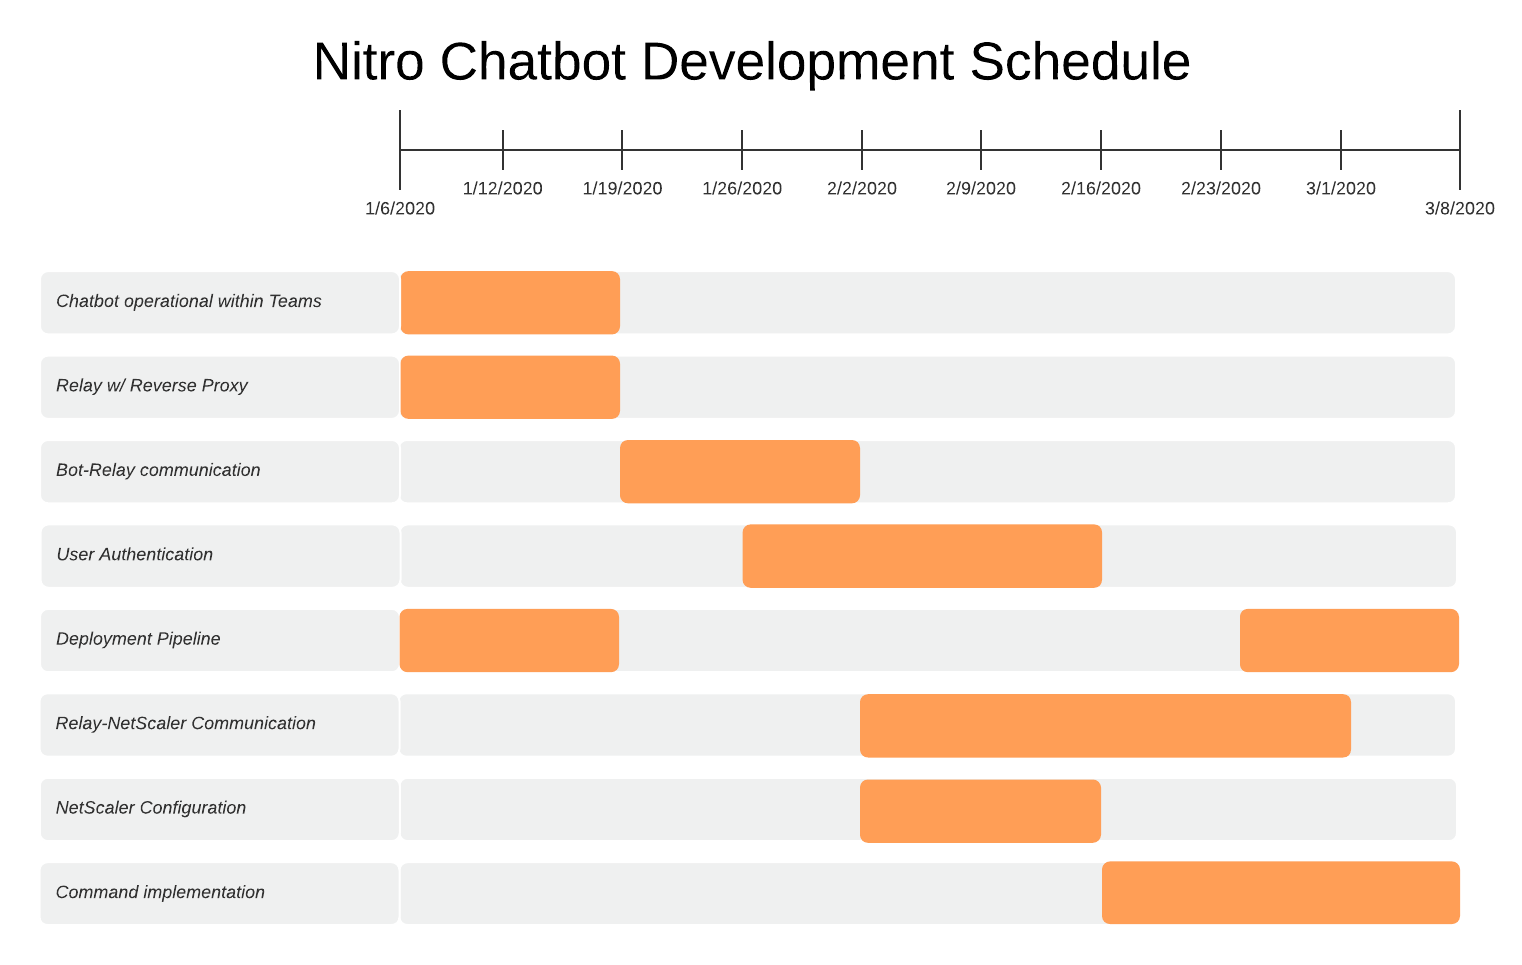
\includegraphics[height=9cm]{gantt.png}
%    \caption[Feature implementation timeline]{This is tentative development schedule for Winter term 2020. This timeline give a rough estimation of when features will be implemented.}
%    \label{fig:Feature implementation Timeline}
%\end{figure}

\clearpage
%\bibliographystyle{IEEEtran}
%\bibliography{dd}
\end{document}